\documentclass[18pt]{article}
\usepackage[utf8]{inputenc}
\usepackage[T1]{fontenc}
\usepackage{ragged2e}
\usepackage{caladea}
\usepackage{graphicx}
\usepackage{longtable}
\usepackage{wrapfig}
\usepackage{rotating}
\usepackage{epigraph}
\usepackage[normalem]{ulem}
\usepackage{hyperref}
\usepackage{amsmath}
\usepackage{amssymb}
\usepackage{capt-of}
\usepackage{hyperref}
\usepackage{fancyhdr}

\title{
 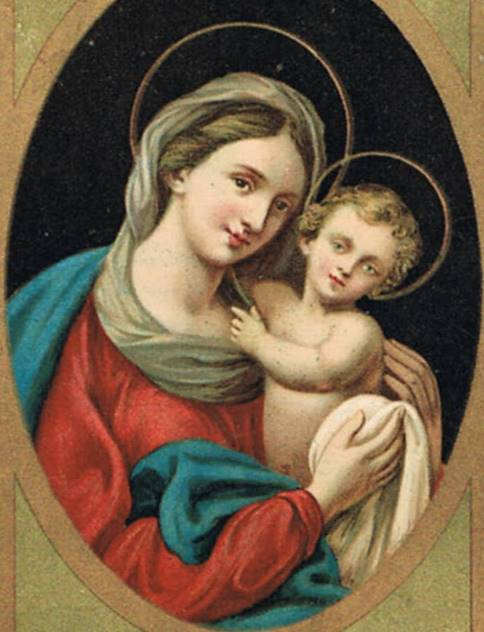
\includegraphics[scale=.9, trim={10cm, 0, 10cm, 0}]{./assets/imagem.jpg}
  \par
   NOVENA A NOSSA SENHORA DA CONFIANÇA}
\date{Início da Novena: 15/02 - Data Litúrgica: 23/02 }

% Comando para fazer "Sumário" não aparecer no Sumário.
\renewcommand{\contentsname}{Sumário}
\begin{document}
\maketitle

\thispagestyle{empty} %zera a primeira página

\pagestyle{fancy}
\fancyhf{} % clear existing header/footer entries
\fancyfoot[LO, CE]{

\includegraphics[scale=0.2]{./assets/cross.png} Nossa Senhora da Confiança, Rogai por nós!
}
% Place Page X of Y on the right-hand
% side of the footer
\fancyfoot[R]{\thepage}

\newpage

\tableofcontents

\centering
\vfill
Visite-nos no Telegram: \url{https://t.me/CotidieNovena}
\newpage

\newpage


%%%%%%%%%%%%%%%%%%%%%%%%%%%%%%%%%%%%% Orações %%%%%%%%%%%%%%%%%%%%%%%%%%%%%%%%%%%%%%%%%%%

\begin{justify}

 \begin{center}
  \section{História}\label{sec:História} % (fold)
 \end{center}

Irmã Clara Isabella Fornari é uma monja clarissa falecida em 1744, cujo processo de beatificação está em andamento. Ela foi privilegiada por Deus com graças místicas, entre as quais a de receber, em seus membros, os estigmas da Paixão.

Irmã Clara sempre foi muito devota de Nossa Senhora e sempre trazia consigo um quadro que a representa com o Menino Jesus nos braços. A essa pintura, foram atribuídas graças e curas numerosas, e, já no século XVIII, começaram a circular pela Itália cópias dela, dando origem à devoção a Santíssima Virgem sob o título de Mãe da Confiança.


\begin{justify}
 \subsection{Do Mosteiro ao Seminário}
\end{justify}

Em 1781, o quadro saiu do Mosteiro a pedido do sobrinho de um padre Jesuíta, padre Crivelli, que sofria de uma grave doença e desejou se penitenciar diante da imagem de Nossa Senhora da Confiança, cuja devoção seu tio lhe transmitira. Ele se curou e, em agradecimento, mandou fazer uma cópia exata do quadro de sua celestial benfeitora.

A cópia da imagem o acompanhou à Roma quando foi designado diretor espiritual do Colégio Germânico, que foi sede, por longo período, do Pontifício Seminário Romano Maior, e Nossa Senhora da Confiança foi eleita padroeira do Seminário.

A sede definitiva do Seminário ficou pronta em 1917 e a nova capela foi dedicada à sua padroeira. O Papa Bento XV, nessa solene ocasião, coroou Nossa Senhora da Confiança, confirmando canonicamente seu título e o dia de sua festa, em 24 de fevereiro.


\begin{justify}
 \subsection{Proteção aos semniaristas}

Nossa Senhora, desde o início, mostrou aos seminaristas que podiam contar com seu poderoso auxilio, sempre que recorressem a Ela sob a invocação de Nossa Senhora da Confiança. Existem dois fatos muito marcantes em que a intercessão da Santíssima Virgem operou milagres entre os seminaristas.

Quando houve uma epidemia de cólera em Roma, o Seminário foi milagrosamente poupado e, além disso, na Primeira Guerra Mundial, cerca de cem seminaristas foram enviados à frente de batalha e se colocaram sob a especial proteção da Nossa Senhora da Confiança.

Todos retornaram vivos, graça que atribuíram à proteção da Santíssima Virgem. Em agradecimento, entronizaram o venerável quadro numa nova capela de mármore e prata.
\end{justify}


\begin{center}
 \subsection*{Créditos:}
\href{https://www.miliciadaimaculada.org.br/colaborador/campanha/historia-de-nossa-senhora-da-confianca}{Milícia da Imaculada}
\end{center}


\end{justify}
%%%%%%%%%%%%%%%%%%%%%%%%%%%%%%%%%%%%% Orações %%%%%%%%%%%%%%%%%%%%%%%%%%%%%%%%%%%%%%%%%%%
\begin{justify}

\newpage
\begin{center}
 \section{Orações}\label{sec:Orações} % (fold)
\textit{Em nome do Pai, e do Filho, e do Espírito Santo. Amém.}
\end{center}


Ó Maria, em vossas mãos ponho essa súplica…
Abençoai-a e depois apresentai-a a Jesus. Fazei valer vosso amor de Mãe e vosso poder de Rainha.
Ó Maria, conto com vosso auxílio; confio em vosso poder.
Entrego-me à vossa vontade. Estou seguro de vossa misericórdia.
Ó Mãe de Deus e minha, rogai por mim. Nossa Senhora da Confiança, rogai por nós. Amém.

\subsection{Oração Final}\label{sec:Oração_Final} % (fold)
\begin{center}
\textbf{Pai Nosso, Ave Maria, Glória ao Pai.}

\vfill
\section*{Nossa Senhora da Confiança, rogai por nós!}

\vfill
\subsection*{Créditos:}
\href{https://rosariopermanente.leiame.net/novena-a-nossa-senhora-da-confianca/}{Movimento do Rosário Permanente}

\end{center}


\end{justify}

\end{document}
